\chapter{Catálisis}\label{ch:g12:catalysis}

Un frasco de agua oxigenada pasa meses en el armario del cuarto de baño
sin alterarse. Vertida sobre una rodilla raspada, hace espuma al
instante: algo en la sangre la descompone en segundos en agua y oxígeno.
Ese algo no se gasta y no aparece en la ecuación de la reacción. Es un
\omterm{def:g12:catalysis:catalyst}{catalizador}. Los \omterm{def:g12:catalysis:catalyst}{catalizadores} hacen posible la mayor parte de la
industria química, limpian los gases de escape de los coches y dirigen
todas las reacciones de la vida.

\begin{recall}
La velocidad de una reacción y los \omterm{def:g12:reaction-rates:kinetic-factor}{factores cinéticos} que la modifican
(\cref{ch:g12:reaction-rates}). Un mecanismo es una serie de \omterm{def:g12:curly-arrows:mechanism}{etapas
elementales}, a través de intermedios (\cref{ch:g12:curly-arrows}).
\end{recall}

\section{Qué es un catalizador}

\begin{definition}[Catalizador, catálisis]\label{def:g12:catalysis:catalyst}
Un \emph{catalizador}\index{catalizador} es una especie que hace más
rápida una reacción sin consumirse: interviene en el mecanismo, pero se
recupera intacto al final, y no aparece en la ecuación global. La
aceleración de una reacción por un catalizador es la
\emph{catálisis}\index{catalisis@catálisis}.
\end{definition}

\begin{proposition}[Un catalizador cambia el camino, no el destino]\label{prop:g12:catalysis:path}
Un \omterm{def:g12:catalysis:catalyst}{catalizador} abre un mecanismo distinto, cuyas barreras de energía son
más bajas que la de la reacción sin catalizar, de modo que una mayor
parte de los encuentros entre partículas tiene éxito. No cambia los
productos formados ni el \omterm{def:g10:reaction-progress-table:system}{estado final} alcanzado; solo lo alcanza antes.
\end{proposition}

\begin{proof}
Se admite: el perfil se estudia en el volumen del primer año. Que el
\omterm{def:g10:reaction-progress-table:system}{estado final} no cambie se deduce de que el \omterm{def:g12:catalysis:catalyst}{catalizador} se recupera: la
reacción global, con sus \omterm{def:g7:chemical-reactions:reactant}{reactivos} y sus productos, es la misma.
\end{proof}

\begin{omfigure}
\begin{minipage}{0.49\linewidth}
\begin{tikzpicture}
\begin{axis}[width=\linewidth, height=5.4cm, xmin=0, xmax=1, ymin=-60,
    ymax=110, xtick=\empty, ytick=\empty, axis lines*=left,
    xlabel={avance de la reacción}, ylabel={energía},
    label style={font=\small}, legend style={font=\scriptsize,
    at={(0.02,0.99)}, anchor=north west, draw=none}, legend cell align=left]
  \addplot[very thick, omDef] table[x=s, y=Eu] {figdata/out/grade-12-catalysis-a.dat};
  \addplot[very thick, omProp] table[x=s, y=Ec] {figdata/out/grade-12-catalysis-a.dat};
  \legend{sin catalizador, con catalizador}
  \node[font=\scriptsize, anchor=north west] at (axis cs:0.02,-4) {reactivos};
  \node[font=\scriptsize, anchor=south east] at (axis cs:0.99,-36) {productos};
\end{axis}
\end{tikzpicture}
\end{minipage}\hfill
\begin{minipage}{0.49\linewidth}
\begin{tikzpicture}
\begin{axis}[width=\linewidth, height=5.4cm, xmin=0, xmax=60, ymin=0,
    ymax=80, xlabel={$t$ (\si{min})}, ylabel={\ce{O2} desprendido (\si{mL})},
    axis lines*=left, ymajorgrids, grid style={gray!20},
    tick label style={font=\scriptsize}, label style={font=\small},
    legend style={font=\scriptsize, at={(0.98,0.03)}, anchor=south east,
    draw=none}, legend cell align=left]
  \addplot[very thick, omDef] table[x=t, y=Vu] {figdata/out/grade-12-catalysis-b.dat};
  \addplot[very thick, omProp] table[x=t, y=Vc] {figdata/out/grade-12-catalysis-b.dat};
  \legend{sin catalizador, con catalizador}
\end{axis}
\end{tikzpicture}
\end{minipage}

{\small Izquierda: la energía a lo largo de la reacción; el camino
catalizado pasa por un intermedio y dos barreras más bajas. Derecha:
oxígeno desprendido por una disolución de peróxido de hidrógeno; el
\omterm{def:g12:catalysis:catalyst}{catalizador} acelera la reacción, pero el volumen final es el mismo.
(Curvas de un modelo.)}
\end{omfigure}

\section{Catálisis homogénea}

\begin{definition}[Catálisis homogénea y heterogénea]\label{def:g12:catalysis:homogeneous}
La \omterm{def:g12:catalysis:catalyst}{catálisis} es una \emph{catálisis homogénea}\index{catalisis homogenea@catálisis homogénea}
cuando el \omterm{def:g12:catalysis:catalyst}{catalizador} está en la misma fase que los \omterm{def:g7:chemical-reactions:reactant}{reactivos} (por
ejemplo, disuelto con ellos), y una \emph{catálisis heterogénea}\index{catalisis heterogenea@catálisis heterogénea}
cuando está en otra fase, normalmente un sólido a cuya superficie llegan
los \omterm{def:g7:chemical-reactions:reactant}{reactivos} desde un gas o un líquido.
\end{definition}

\begin{example}[Los iones yoduro y el peróxido de hidrógeno]\label{ex:g12:catalysis:iodide}
El peróxido de hidrógeno se descompone muy despacio por sí solo:
\ce{2H2O2 -> 2H2O + O2}. Con un poco de yoduro de potasio disuelto,
hace espuma al instante. El \omterm{def:g9:ions:ion}{ion} yoduro abre un camino en dos etapas:
\[
  \ce{H2O2 + I- -> H2O + IO-}, \qquad
  \ce{H2O2 + IO- -> H2O + O2 + I-} .
\]
Sumadas, las dos etapas devuelven \ce{2H2O2 -> 2H2O + O2}: el \omterm{def:g9:ions:ion}{ion} yoduro,
consumido en la primera etapa y recuperado en la segunda, es el
\omterm{def:g12:catalysis:catalyst}{catalizador}; el \omterm{def:g9:ions:ion}{ion} \ce{IO-} es un intermedio.
\end{example}


\begin{example}[Los iones hierro(III)]\label{ex:g12:catalysis:iron}
Los \omterm{def:g9:ions:ion}{iones} hierro(III) también catalizan la descomposición, a través del
par \ce{Fe^{3+}}/\ce{Fe^{2+}} (\cref{ch:g11:redox}): primero oxidan el
peróxido de hidrógeno, \ce{2Fe^{3+} + H2O2 -> 2Fe^{2+} + O2 + 2H+}, y
después los \omterm{def:g9:ions:ion}{iones} hierro(II) formados vuelven a oxidarse con más
peróxido de hidrógeno,
\ce{2Fe^{2+} + H2O2 + 2H+ -> 2Fe^{3+} + 2H2O}. El color naranja pálido
de la disolución vira a verdoso mientras se desprende el gas, y vuelve
cuando se agota el peróxido de hidrógeno: señal de que el \omterm{def:g12:catalysis:catalyst}{catalizador}
interviene y se regenera.
\end{example}

\section{Catálisis heterogénea}

Muchos \omterm{def:g12:catalysis:catalyst}{catalizadores} industriales son sólidos: \omterm{def:g9:periodic-table-first-look:metal}{metales} como el platino,
el paladio, el níquel o el hierro, u óxidos. La reacción tiene lugar en
su superficie, en tres fases: las \omterm{def:g7:atoms-and-molecules:molecule}{moléculas} de \omterm{def:g7:chemical-reactions:reactant}{reactivo} quedan retenidas
en la superficie (adsorbidas), donde sus enlaces se debilitan;
reaccionan allí; los productos abandonan la superficie, que queda libre
para nuevas \omterm{def:g7:atoms-and-molecules:molecule}{moléculas}. Por eso un \omterm{def:g12:catalysis:catalyst}{catalizador} se fabrica con la mayor
superficie posible: polvo fino, o una capa delgada sobre un soporte
poroso.

\begin{omfigure}
\begin{tikzpicture}[font=\small]
  \foreach \x in {0,4.2,8.4} {
    \fill[black!25] (\x,0) rectangle (\x+3.4,0.35);
    \foreach \i in {0,1,2,3,4,5,6,7} \shade[ball color=black!35] (\x+0.21+\i*0.425,0.35) circle (0.2);
  }
  % 1. adsorption
  \node[aH, minimum size=3.2mm] at (0.9,0.75) {};
  \node[aH, minimum size=3.2mm] at (1.3,0.75) {};
  \node[aH, minimum size=3.2mm] (h1) at (2.2,1.8) {};
  \node[aH, minimum size=3.2mm] (h2) at (2.6,1.8) {};
  \draw[bond, line width=1.2pt] (h1.east) -- (h2.west);
  \draw[->, omProp, thick] (2.4,1.55) -- (2.0,1.0);
  \node[anchor=north, align=center] at (1.7,-0.1) {1. adsorción:\\ el enlace \ce{H-H} se rompe};
  % 2. reaction on the surface
  \node[aC] (c1) at (5.5,1.05) {}; \node[aC] (c2) at (6.2,1.05) {};
  \draw[bond, line width=1.4pt] (c1) -- (c2);
  \node[aH, minimum size=3.2mm] at (5.3,0.75) {};
  \node[aH, minimum size=3.2mm] at (6.6,0.75) {};
  \node[anchor=north, align=center] at (5.9,-0.1) {2. los átomos H se unen\\ a la molécula adsorbida};
  % 3. desorption
  \node[aC] (c3) at (9.6,1.8) {}; \node[aC] (c4) at (10.3,1.8) {};
  \draw[bond, line width=1.4pt] (c3) -- (c4);
  \foreach \a/\c in {150/c3,210/c3,90/c3,30/c4,-30/c4,90/c4}
    \node[aH, minimum size=2.8mm] at ($(\c)+(\a:0.42)$) {};
  \draw[->, omProp, thick] (11.0,1.2) -- (11.0,2.2);
  \node[anchor=north, align=center] at (10.1,-0.1) {3. el producto\\ abandona la superficie};
\end{tikzpicture}

{\small Adición de hidrógeno al eteno sobre una superficie metálica:
adsorción, reacción, desorción. El \omterm{def:g9:periodic-table-first-look:metal}{metal} se recupera intacto.}
\end{omfigure}

\begin{example}[El convertidor catalítico]\label{ex:g12:catalysis:converter}
Los gases de escape de un motor de gasolina contienen monóxido de
carbono y monóxido de nitrógeno, ambos tóxicos, y \omterm{def:g4:what-a-fire-needs:fuel}{combustible} sin
quemar. En el convertidor catalítico, un panal cerámico recubierto de
platino y rodio, reaccionan sobre la superficie del \omterm{def:g9:periodic-table-first-look:metal}{metal}:
\[
  \ce{2CO + 2NO -> 2CO2 + N2} ,
\]
y los hidrocarburos se queman dando dióxido de carbono y agua. Los gases
atraviesan el convertidor en una fracción de segundo, demasiado deprisa
para que ocurra ninguna reacción sin \omterm{def:g12:catalysis:catalyst}{catalizador}.
\end{example}

\begin{omfigure}
\begin{tikzpicture}[font=\small]
  \fill[black!12, draw=black!60, rounded corners=6pt] (0,0) rectangle (6,2.4);
  \foreach \x in {0.3,0.6,0.9,1.2,1.5,1.8,2.1,2.4,2.7,3.0,3.3,3.6,3.9,4.2,4.5,4.8,5.1,5.4,5.7} \draw[black!35] (\x,0.2) -- (\x,2.2);
  \foreach \y in {0.5,0.9,1.3,1.7,2.1} \draw[black!35] (0.2,\y) -- (5.8,\y);
  \fill[black!40] (-1.4,0.9) rectangle (0,1.5);
  \fill[black!40] (6,0.9) rectangle (7.4,1.5);
  \draw[->, very thick, omThm] (-2.6,1.2) -- (-1.5,1.2);
  \node[anchor=east, align=right, omThm] at (-2.7,1.2) {\ce{CO}, \ce{NO},\\ hidrocarburos};
  \draw[->, very thick, omMeth] (7.5,1.2) -- (8.6,1.2);
  \node[anchor=west, align=left, omMeth] at (8.7,1.2) {\ce{CO2}, \ce{N2},\\ \ce{H2O}};
  \node[align=center, fill=white, inner sep=2pt] at (3,1.2) {panal cerámico\\ recubierto de Pt y Rh};
\end{tikzpicture}

{\small Un convertidor catalítico cortado longitudinalmente: miles de
canales finos ofrecen a los gases de escape una superficie enorme
recubierta de \omterm{def:g9:periodic-table-first-look:metal}{metal}.}
\end{omfigure}

\begin{omfigure}
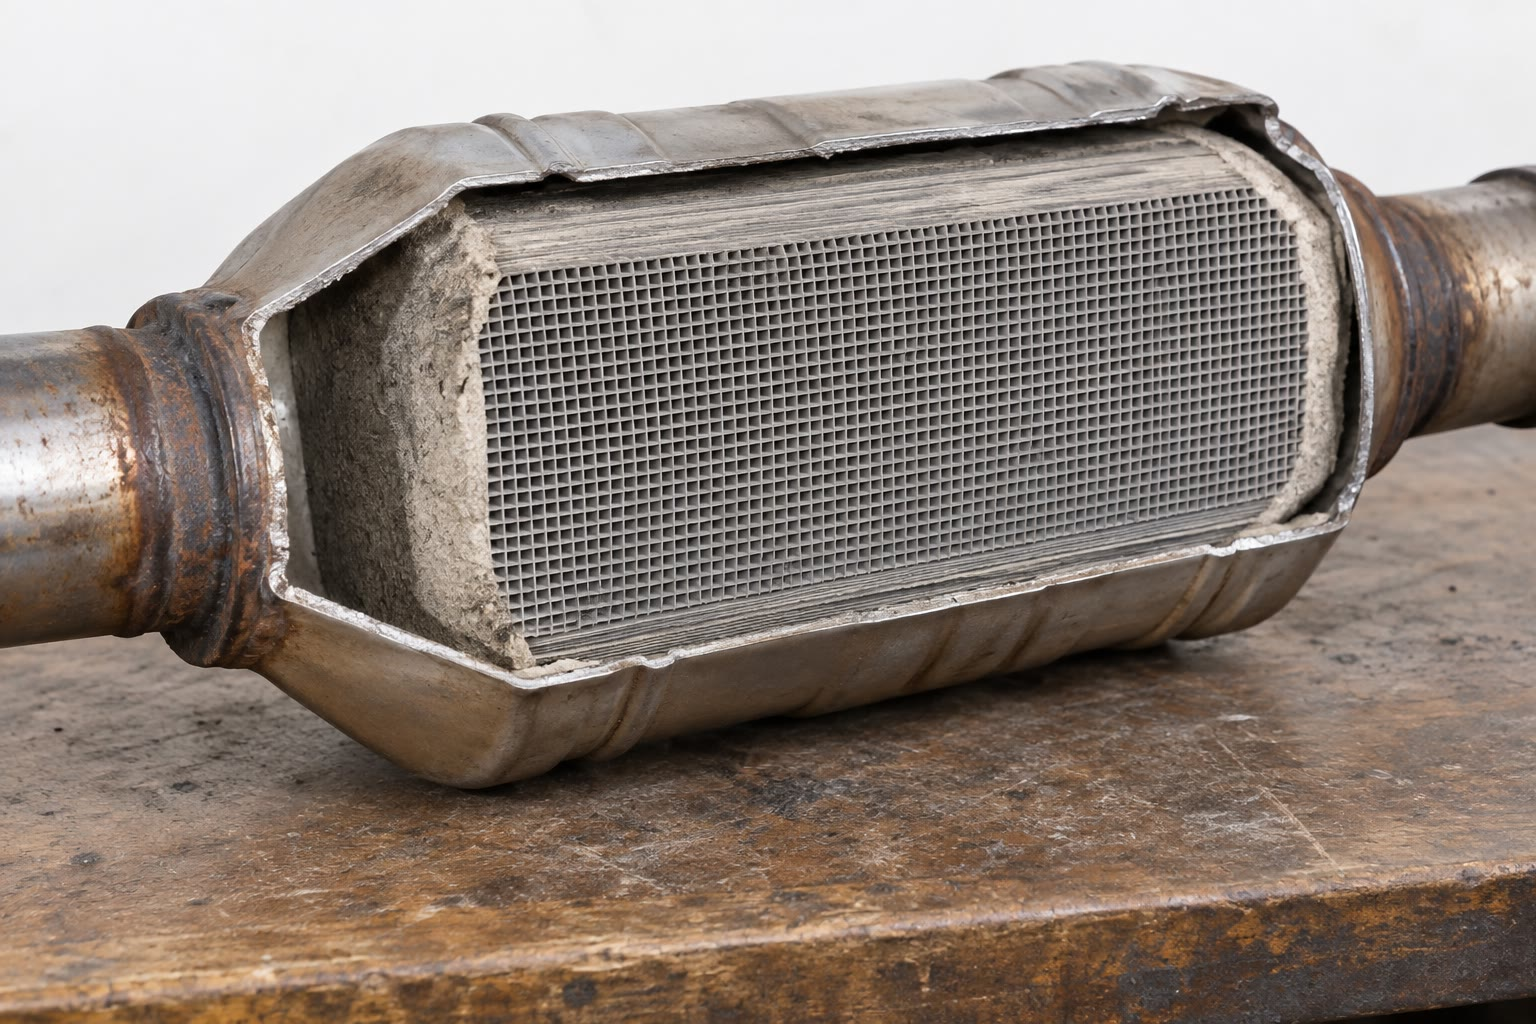
\includegraphics[width=0.45\linewidth]{images/book1/ai/g12-catalytic-converter.jpg}

{\small Un convertidor catalítico abierto: el \omterm{def:g9:inside-the-atom:nucleus}{núcleo} en panal.}
\end{omfigure}

\begin{history}[Haber, Bosch y el amoníaco]
% ledger: haber:T, haber:p, nh3:world-2024
A principios del siglo XX, el químico Fritz Haber descubrió cómo combinar
el nitrógeno del \omterm{def:g4:air-a-mixture-of-gases:air}{aire} con hidrógeno, \ce{N2 + 3H2 -> 2NH3}, sobre un
\omterm{def:g12:catalysis:catalyst}{catalizador} a base de hierro, y el ingeniero Carl Bosch lo convirtió en
un proceso industrial. Hoy sigue funcionando a entre 400 y
\qty{500}{\celsius} y entre 150 y \qty{250}{atm}. En 2024, el mundo
produjo amoníaco con unos 150 millones de toneladas de nitrógeno, la
mayor parte para fertilizantes: una gran parte del nitrógeno de los
alimentos que comemos ha pasado por un \omterm{def:g12:catalysis:catalyst}{catalizador} así.
\end{history}

\section{Enzimas}

\begin{definition}[Enzima]\label{def:g12:catalysis:enzyme}
Una \emph{enzima}\index{enzima} es una proteína fabricada por un ser vivo
que cataliza una reacción de su química. Las enzimas son muy eficaces y
muy específicas: cada una solo encaja con unas pocas \omterm{def:g7:atoms-and-molecules:molecule}{moléculas}, y
funcionan mejor en un intervalo estrecho de temperatura y de acidez.
\end{definition}

\begin{example}[La catalasa]\label{ex:g12:catalysis:catalase}
El peróxido de hidrógeno se forma en las células como subproducto y les
resulta dañino. La \omterm{def:g12:catalysis:enzyme}{enzima} catalasa, presente en la sangre, el hígado y
muchos tejidos vegetales, lo descompone en agua y oxígeno a una
velocidad enorme: es la espuma de una rodilla raspada, o la de una
rodaja de patata cruda. La patata cocida no hace espuma: el calor ha
destruido la forma de la \omterm{def:g12:catalysis:enzyme}{enzima}.
\end{example}

\begin{omfigure}
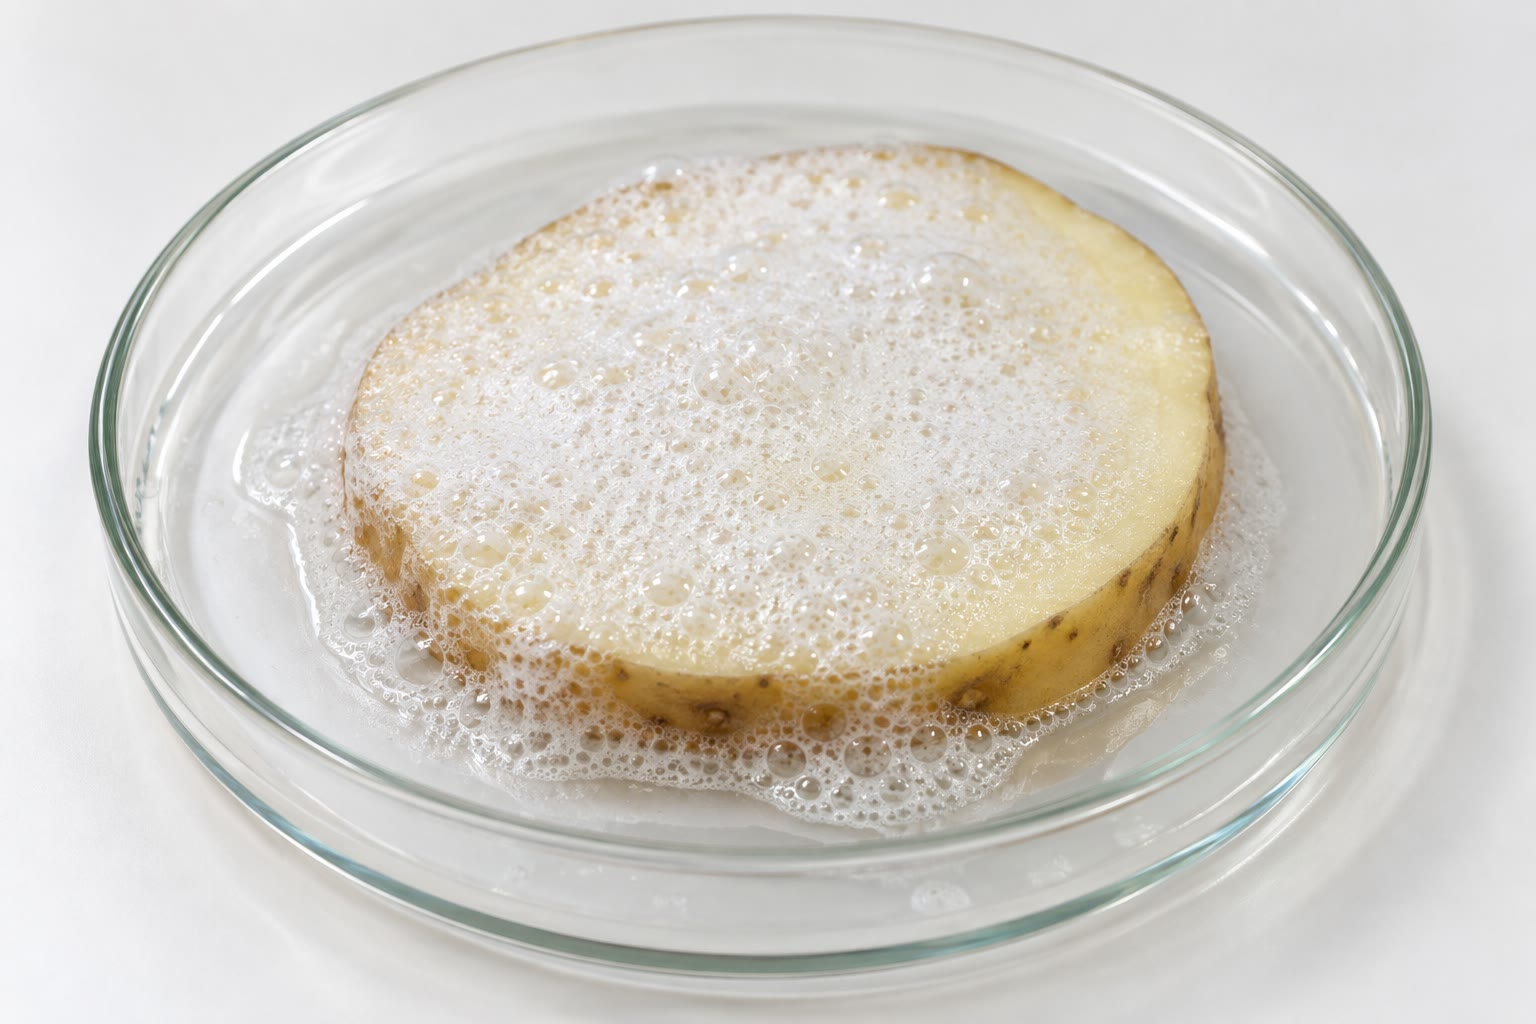
\includegraphics[width=0.45\linewidth]{images/book1/ai/g12-potato-peroxide.jpg}

{\small Agua oxigenada sobre una rodaja de patata cruda: la catalasa en
acción.}
\end{omfigure}

\section{Selectividad}

\begin{definition}[Catalizador selectivo]\label{def:g12:catalysis:selective}
Cuando los mismos \omterm{def:g7:chemical-reactions:reactant}{reactivos} pueden dar varias reacciones, un
\emph{catalizador selectivo}\index{catalizador selectivo} acelera una de
ellas mucho más que las otras, y así decide qué productos se forman.
\end{definition}

\begin{example}[Dos destinos del etanol]\label{ex:g12:catalysis:ethanol}
El vapor de etanol caliente que pasa sobre alúmina pierde agua y da
eteno, \ce{C2H5OH -> C2H4 + H2O} (una \omterm{def:g12:curly-arrows:categories}{eliminación}); al pasar sobre cobre
caliente, pierde hidrógeno y da etanal, \ce{C2H5OH -> CH3CHO + H2}. El
mismo \omterm{def:g7:chemical-reactions:reactant}{reactivo}, dos \omterm{def:g12:catalysis:catalyst}{catalizadores}, dos productos.
\end{example}

\begin{remark}[La industria y la vida funcionan con catalizadores]\label{rem:g12:catalysis:everywhere}
La mayoría de los productos de la industria química, desde los
\omterm{def:g4:what-a-fire-needs:fuel}{combustibles} hasta los \omterm{def:g8:plastics:plastic}{plásticos} y los fertilizantes, se fabrican con
\omterm{def:g12:catalysis:catalyst}{catalizadores}; encontrar un \omterm{def:g12:catalysis:catalyst}{catalizador} más activo o más selectivo ahorra
energía y residuos. Cada reacción de una célula viva está catalizada por
una \omterm{def:g12:catalysis:enzyme}{enzima}.
\end{remark}

\begin{safety}{\ghs[0.82cm]{GHS03}\ghs[0.82cm]{GHS05}\ghs[0.82cm]{GHS07}}
% ledger: ghs:H2O2
El peróxido de hidrógeno concentrado es un \omterm{def:g11:redox:oxidant}{oxidante} fuerte que puede
avivar un incendio, quema la piel y los ojos y es nocivo si se ingiere.
Las disoluciones diluidas del laboratorio también exigen gafas y
guantes; la descomposición libera oxígeno, así que nunca se hace en un
recipiente cerrado.
\end{safety}

\section{Ejercicios}


\begin{exercise}[$\star$]\label{exo:g12:catalysis:1}
En la descomposición del peróxido de hidrógeno catalizada por \omterm{def:g9:ions:ion}{iones}
yoduro, ¿qué especies son \omterm{def:g7:chemical-reactions:reactant}{reactivos}, cuáles productos, cuál es el
\omterm{def:g12:catalysis:catalyst}{catalizador} y cuál un intermedio?
\end{exercise}

\begin{exercise}[$\star$]\label{exo:g12:catalysis:2}
¿\omterm{def:g12:catalysis:homogeneous}{Catálisis homogénea} o heterogénea?: \omterm{def:g9:ions:ion}{iones} yoduro en una disolución de
peróxido de hidrógeno; platino en un convertidor catalítico; hierro en la
\omterm{def:g10:synthesis-yield:synthesis}{síntesis} del amoníaco; \omterm{def:g9:ions:ion}{iones} hierro(III) en una disolución de peróxido de
hidrógeno.
\end{exercise}

\begin{exercise}[$\star$]\label{exo:g12:catalysis:3}
En los perfiles de energía, ¿qué camino tiene la barrera más alta? ¿Son
iguales las energías inicial y final en ambos caminos? ¿Qué significa
esto para los productos?
\end{exercise}

\begin{exercise}[$\star$]\label{exo:g12:catalysis:4}
¿Por qué un \omterm{def:g12:catalysis:catalyst}{catalizador} no aparece en la ecuación global de una reacción?
\end{exercise}

\begin{exercise}[$\star$]\label{exo:g12:catalysis:5}
¿Por qué los \omterm{def:g12:catalysis:catalyst}{catalizadores} sólidos de la industria se usan como polvos
finos o como capas delgadas sobre soportes porosos?
\end{exercise}

\begin{exercise}[$\star\star$]\label{exo:g12:catalysis:6}
Suma las dos etapas de la descomposición del peróxido de hidrógeno
catalizada por hierro(III) y demuestra que los \omterm{def:g9:ions:ion}{iones} hierro y los \omterm{def:g9:ions:ion}{iones}
hidrógeno se simplifican.
\end{exercise}

\begin{exercise}[$\star\star$]\label{exo:g12:catalysis:7}
Lee las curvas del oxígeno desprendido. ¿Cuánto tarda cada ensayo en
liberar la mitad del volumen final? ¿Por qué factor lo acorta el
\omterm{def:g12:catalysis:catalyst}{catalizador}?
\end{exercise}

\begin{exercise}[$\star\star$]\label{exo:g12:catalysis:8}
En los coches equipados con convertidor catalítico no se usa gasolina con
plomo: el plomo se deposita sobre el platino y se queda allí. Explica por
qué esto estropea el convertidor, aunque la reacción normal no consuma el
platino.
\end{exercise}

\begin{exercise}[$\star\star$]\label{exo:g12:catalysis:9}
Un alumno mide la espuma producida por rodajas de patata en agua
oxigenada a 10, 25, 37, 60 y \qty{80}{\celsius}: la espuma aumenta hasta
unos \qty{37}{\celsius}, luego disminuye y casi desaparece a
\qty{80}{\celsius}. Explica las dos partes de la curva.
\end{exercise}

\begin{exercise}[$\star\star$]\label{exo:g12:catalysis:10}
Escribe la ecuación de la reacción entre el monóxido de carbono y el
monóxido de nitrógeno en un convertidor catalítico y comprueba que está
ajustada. ¿Por qué se eliminan los dos contaminantes a la vez?
\end{exercise}

\begin{exercise}[$\star\star$]\label{exo:g12:catalysis:11}
\qty{10.0}{mL} de una disolución de peróxido de hidrógeno desprenden
\qty{72}{mL} de oxígeno a \qty{20}{\celsius} al descomponerse por
completo. Calcula la cantidad de oxígeno ($V_m = \qty{24.1}{L/mol}$) y
después la concentración de peróxido de hidrógeno de la disolución.
\end{exercise}

\begin{exercise}[$\star\star\star$]\label{exo:g12:catalysis:12}
El vapor de etanol que pasa sobre alúmina da eteno; sobre cobre da
etanal. Escribe las dos ecuaciones, indica la categoría de la primera y
explica qué es un \omterm{def:g12:catalysis:selective}{catalizador selectivo}.
\end{exercise}

\begin{exercise}[$\star\star\star$]\label{exo:g12:catalysis:13}
Un \omterm{def:g12:catalysis:catalyst}{catalizador} hace una reacción diez veces más rápida. Un alumno afirma
que también da diez veces más producto. Corrige la afirmación con ayuda
de las curvas del oxígeno desprendido.
\end{exercise}

\begin{exercise}[$\star\star\star$]\label{exo:g12:catalysis:14}
Una \omterm{def:g7:atoms-and-molecules:molecule}{molécula} de catalasa descompone unos pocos millones de \omterm{def:g7:atoms-and-molecules:molecule}{moléculas} de
peróxido de hidrógeno por segundo. Tomando $\num{5e6}$ por segundo,
¿cuánto tarda una \omterm{def:g7:atoms-and-molecules:molecule}{molécula} de \omterm{def:g12:catalysis:enzyme}{enzima} en descomponer un \omterm{def:g10:the-mole:amount}{mol} de peróxido de
hidrógeno? ¿Cuántas \omterm{def:g7:atoms-and-molecules:molecule}{moléculas} de \omterm{def:g12:catalysis:enzyme}{enzima} lo harían en un segundo? (Un
cálculo de órdenes de magnitud; la velocidad es un dato del ejercicio.)
\end{exercise}

\begin{exercise}[$\star\star\star$]\label{exo:g12:catalysis:15}
% ledger: nh3:world-2024
En 2024, el mundo produjo unos 150 millones de toneladas de nitrógeno en
forma de amoníaco. ¿Qué masa de amoníaco es eso? ¿Qué cantidad de
dinitrógeno se combinó?
\end{exercise}

\section{Problema: el agua oxigenada de la peluquería}

\begin{problem}[{Problema de fin de semana --- ¿cuál es la concentración del
agua oxigenada de ``20 volúmenes''?}]
\label{pb:g12:catalysis:1}
% ledger: const:Vm1, ghs:H2O2, aw:H, aw:O
En las peluquerías se usan disoluciones de peróxido de hidrógeno
etiquetadas en ``volúmenes'': una disolución de ``20 volúmenes'' es
aquella de la que \qty{1}{L} desprende \qty{20}{L} de oxígeno al
descomponerse por completo, midiendo el gas a \qty{0}{\celsius} y a la
presión atmosférica normal, donde un \omterm{def:g10:the-mole:amount}{mol} de gas ocupa \qty{22.4}{L}.

\medskip
\noindent\textbf{Parte I --- La descomposición.}
\begin{enumerate}
  \item Escribe la ecuación de la descomposición del peróxido de
        hidrógeno.
  \item ¿Es la descomposición una \omterm{def:g11:redox:reaction}{reacción redox}? Encuentra el \omterm{def:g11:redox:oxidant}{oxidante} y
        el \omterm{def:g11:redox:oxidant}{reductor} (el peróxido de hidrógeno es ambos).
  \item ¿Por qué se conserva un frasco durante meses, aunque la reacción
        sea posible?
\end{enumerate}

\medskip
\noindent\textbf{Parte II --- Qué significa ``20 volúmenes''.}
\begin{enumerate}[resume]
  \item ¿Qué cantidad de oxígeno desprende \qty{1}{L} de la disolución?
  \item Deduce la cantidad de peróxido de hidrógeno en \qty{1}{L}.
  \item Da la \omterm{def:g10:concentration-and-dilution:molar-concentration}{concentración molar}.
  \item Calcula la \omterm{def:g10:the-mole:molar-mass}{masa molar} del peróxido de hidrógeno y la
        \omterm{def:g10:concentration-and-dilution:mass-concentration}{concentración en masa}.
  \item ¿Qué significaría ``10 volúmenes'' en \omterm{def:g10:the-mole:amount}{moles} por litro?
\end{enumerate}

\medskip
\noindent\textbf{Parte III --- Dos \omterm{def:g12:catalysis:catalyst}{catalizadores}.}
\begin{enumerate}[resume]
  \item Se añade a una muestra una gota de sangre (catalasa) y a otra
        unas gotas de cloruro de hierro(III). ¿Qué tipo de \omterm{def:g12:catalysis:catalyst}{catálisis} es
        cada una?
  \item Escribe las dos etapas de la \omterm{def:g12:catalysis:catalyst}{catálisis} por hierro(III) y
        comprueba que su suma es la descomposición.
  \item Con las curvas del oxígeno desprendido, describe cómo cambia el
        volumen de oxígeno con y sin \omterm{def:g12:catalysis:catalyst}{catalizador}, y qué permanece igual.
  \item ¿Por qué el color de una muestra catalizada por hierro(III)
        cambia durante la reacción y vuelve al final?
  \item ¿Por qué una patata cocida no hace espumar la disolución?
\end{enumerate}

\medskip
\noindent\textbf{Parte IV --- El frasco.}
\begin{enumerate}[resume]
  \item ¿Qué volumen de oxígeno, medido a \qty{0}{\celsius}, puede
        desprender un frasco de \qty{100}{mL}?
  \item ¿Qué volumen es eso a \qty{20}{\celsius} ($V_m =
        \qty{24.1}{L/mol}$)?
  \item ¿Por qué el tapón de un frasco así debe dejar escapar el gas
        lentamente?
  \item Un frasco almacenado durante mucho tiempo se valora y se encuentra
        que contiene \qty{1.50}{mol/L}. ¿Cuántos ``volúmenes'' son ahora?
  \item ¿Qué fracción del peróxido de hidrógeno se ha descompuesto?
  \item Da la respuesta final: ¿cuál es la \omterm{def:g10:concentration-and-dilution:molar-concentration}{concentración molar} de una
        disolución de peróxido de hidrógeno de ``20 volúmenes''?
\end{enumerate}
\end{problem}
